\documentclass{beamer}
\usepackage{etex}
\usetheme{Antibes}
\usepackage{amssymb,amsmath,amsthm}
\usepackage{graphicx}
\usepackage{caption}
\usepackage{subfig}
\newcommand{\bn}{\begin{enumerate}[i)]}
\newcommand{\en}{\end{enumerate}}
\newcommand{\im}{\item}
\newcommand{\CPT}[1]{\large{\textbf{CHAPTER #1}}}
\newcommand{\ir}[1]{\textbf{Remark #1}}
\newcommand{\ith}[1]{\textbf{Theorem #1}}
\newcommand{\idf}[1]{\textbf{Definition #1}}
\newcommand{\iex}[1]{\textbf{Example #1}}

%\definecolor{cardinal}{rgb}{0.77, 0.12, 0.23}
%\usecolortheme[named=cardinal]{structure}
%\setbeamercolor{block title}{bg=cardinal,fg=black}
 \usepackage{tikz}
 \usetikzlibrary{patterns,snakes,plotmarks}
 \usepackage{multirow}
% \usetikzlibrary{shadows}
\usepackage{epstopdf}
\usepackage{nicefrac}
\usepackage{lmodern}
\usepackage{pgfplots}
\usepackage{qtree}
\newcommand*{\Scale}[2][4]{\scalebox{#1}{\ensuremath{#2}}}%
\DeclareCaptionLabelSeparator{horse}{:\,\,} % change according to your needs
\captionsetup{
  labelsep = horse,
  figureposition = bottom % used to get the correct vertical space between the figure and the caption
}
\setbeamertemplate{caption}[numbered]
\setbeamertemplate{items}[circle]
\setbeamertemplate{enumerate items}[square]
\theoremstyle{definition}
\newtheorem*{exs}{Examples}
\newtheorem{ex}{Example}
\newtheorem*{exc}{Exercise}
%\usepackage{booktabs}
\setlength{\parindent}{0pt}
%\setbeameroption{show notes}
 \setbeamerfont{note page}{size=\tiny}
%\setbeamertemplate{note page}[plain]
%\setbeameroption{show only notes}
\title{Math 629 - Survival Analysis \\ Chapter 4: Evaluating the Proportional Hazards Assumption}
\author{Drew Lazar}
\institute{Ball State University}
\date{\today}

\begin{document}
\begin{frame}
    \titlepage
\end{frame}



\section{Chapter 4}
\begin{frame}
\frametitle{Overview of Evaluating PH Assumption}
\begin{block}{Approaches for assessing PH assumption}
\begin{enumerate}
\item Graphical techniques
\begin{enumerate}[i.]
\item Inspect $-\ln(-\ln(\hat{S}))$ survival curves for specifications of covariates of interest.
\item Comparing observed (stratified KM) and expected (Cox PH model) survival curves.
\end{enumerate}
\item Goodness of fit (GOF) techniques. Conduct test of $H_0: \text{Cox PH assumption met}$ and get a $p$-value.
\item Use time-dependent variables in an extended Cox PH model. Test for interaction between these variables and covariates.
\end{enumerate}
\end{block}
\end{frame}
\begin{frame}
\frametitle{Graphical Approaches}
\begin{block}{Log-Log Plots}
Assume Cox PH is met so that
\[ S(t,X) = S_0(t)^{\exp(X'\beta)} \text{ for some }  \beta \in \mathbb{R}^{p\times1}
\]
Then we have
\begin{align*}
&\ln( S(t,X)) = \exp(X'\beta)\ln(S_0(t)) \\
&\implies -\ln(-\ln(S(t,X))) = -\ln(-\ln(-S_0(t))) - X'\beta
\end{align*}
\end{block}
\end{frame}

\begin{frame}
\frametitle{Graphical Approaches (cont'd)}
\begin{block}{Graphical Approach I: Log-Log Plots}
Thus, if population satisfies Cox PH model, for any $X$ and $X^*$,
\begin{align*}
&-\ln(-\ln(S(t,X)))- (-\ln(-\ln(S(t,X^*)))) = \\
&-X'\beta - (-{X^*}'\beta) =(X^*-X)'\beta
\end{align*}
\end{block}
As this expression does not involve time, the  $-\ln(-\ln)$ plots of our survival curves for $X$ and $X^*$, respectively, should be at the same distance throughout the study and their graphs should be parallel. $-\ln(-\ln)$ plots of good estimates, $\hat{S}(t,X)$ and $\hat{S}(t,X^*)$, should exhibit the same behavior if the PH assumption is met. 
\end{frame}

\begin{frame}
\frametitle{Graphical Approaches (cont'd)}
\begin{block}{Problem 4.1 - Log-Log Plots}
For the Remission data, test the Cox PH assumption by using log-log plots and by considering the covariates ``one at a time''.
\begin{enumerate}
\item Test Cox Ph assumption for TR.
\item Test the Cox Ph assumption of LogWBC. First statify LogWbc with low - 1.45 to 2.30, med - 2.31 to 3.00, high 3.01 to 5.00.
\item Test the Cox Ph for Sex.
\end{enumerate}
\end{block}
\end{frame}

\begin{frame}
\frametitle{Graphical Approaches (cont'd)}
\begin{block}{Considerations about Log-Log Plots}
\begin{enumerate}
\item  One might ask "How parallel is parrel enough?". Determining parallelism is based on inspection and is subjective.
\item  For continuous variables such as LogWBC once must choose ``cut-points''. Want many cut-points, but if choose too many data ``thins'' out.
\item  To fully test Cox PH model must choose every combination of classes of covariates. Data might ``thin out'' in this case so test is not reliable (see next slide).
\end{enumerate}
\end{block}
\end{frame}


\begin{frame}
\frametitle{Graphical Approaches (cont'd)}
\begin{block}{Considerations about Log-Log Plots (cont'd)}
\begin{columns}
    \begin{column}{0.48\textwidth}
        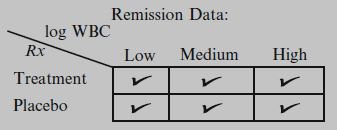
\includegraphics[width =\textwidth, height=4cm]{CH4_loglogMC.JPG}
    \end{column}
    \hspace{-10pt}
    \begin{column}{0.48\textwidth}
         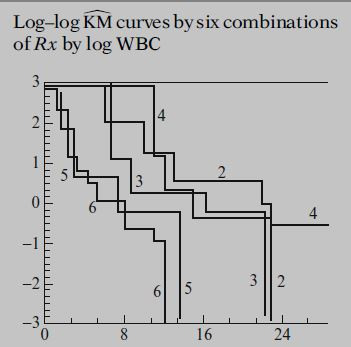
\includegraphics[width =\textwidth, height=5.5cm]{Ch4_loglog6.JPG}
          Plot suggests Cox PH not satisfied, but unreliable.
    \end{column}
\end{columns}
\end{block}
\end{frame}

\begin{frame}
\frametitle{Graphical Approaches (cont'd)}
\begin{block}{Problem 4.2 - Alternative approach to Log-Log plots}
\begin{itemize}
\item Rather than use KM plots on strata, we can fit Cox PH models using covariates that already satisfy the PH assumption.
\item These PH models are fit on strata of covariates we are testing.
\item We then check log-log plots of estimated survival curves from different stata.  We use representative values (eg. overall mean) of covariates which we included in Cox PH model.
\end{itemize}
Use the approach above, assuming LogWBC satisfies the Cox PH model, to test whether TR and Sex satisfy the Cox PH assumption.
\end{block}
\end{frame}

\begin{frame}
\frametitle{Graphical Approaches (cont'd)}
\begin{block}{Graphical Approach II: Observed vs. Expected Plots}
\begin{enumerate}
\item Stratify the data on specifications of covariates that we wish to assess for the PH assumption.
\item Compute and plot KM estimates on these strata. These are our ``observed'' survival curves.
\item Fit a Cox PH model and obtain adjusted survival curves for those specifications. There are our ``expected'' curves.
\item The ``observed'' survival curves should be similar to the ``expected'' curves if the PH assumption holds.
\end{enumerate}
\end{block}
\end{frame}

\begin{frame}
\frametitle{Graphical Approaches (cont'd)}
\begin{block}{Problem 4.3 - Observed vs. Expected Plots}
\begin{enumerate}
\item Test the Cox PH assumption ``one-at-time" on each covariate in the Remission data set (TR, LogWBC, Sex).
\item As LogWBC is continuous we need to 1) choose strata for logWBC and 2) choose a way to represent strata in our Cox PH, ``expected", survival curves. In regard to 2) there are two options
\begin{enumerate}
\item Fit a Cox PH model and choose representative values for each strata (e.g. the means in each strata).
\item Use categorical or ``dummy'' variables for the strata and then fit the Cox PH model. Also, interpret the coefficients of the Cox PH model with dummy variables for level of LogWBC. 
\end{enumerate}
\end{enumerate}
\end{block}
\end{frame}

\begin{frame} 
\frametitle{The Goodness of Fit (GOF) Testing Approach}
\begin{block}{Overview}
\begin{itemize} 
\item A GOF testing approach provides a test statistic and p-value for
assessing the PH assumption for a given predictor of interest.
\item A researcher can make a more objective decision than using a statistical testwhen using either of
the two graphical approaches
\item A number of different tests for assessing the PH
assumption have been proposed in the literature.
\item We consider a test  based on residuals
defined by Schoenfeld (1982), now called the Schoenfeld
residuals.
\end{itemize} 
\end{block}
\end{frame} 

\begin{frame}
\frametitle{The Goodness of Fit (GOF) Testing Approach (cont'd)}
\begin{block}{Schoenfeld Residuals}
\begin{enumerate}
\item For each predictor in the model, Schoenfeld
residuals are defined for every subject who
has an event.
\item If the PH assumption holds for a particular covariate
then the Schoenfeld residuals for that
covariate will not be related to survival time.
\item The null hypothesis is $H_0: \text{The PH assumption holds for a particular covariate}$. 
\item The test statistic is the correlation between Shoenfeld residuals for that covariate and ordered event times. 
\end{enumerate} 
\end{block}
\end{frame} 

\begin{frame} 
\frametitle{The Goodness of Fit (GOF) Testing Approach (cont'd)}
\begin{block}{Problem 4.4 - Using Schoenfeld residuals to test PH assumption}
For the Remission data set, use Schoenfeld residuals to test the PH assumption for
\begin{enumerate}
\item just TR, 
\item TR and logWBC simultaneously and 
\item TR, LogWBC and Sex simultaneously. 
\end{enumerate} 
\end{block}
\end{frame} 


\end{document} 